  

\begin{figure}
\begin{center}
\begin{tikzpicture}[thick,action/.style={shape=rectangle, rounded corners,
                     draw, anchor=center,
                     text width=10em, align=center,
                     top color=white, bottom color=blue!20,
                     inner sep=1ex},
                   model/.style={shape=circle,
                     draw, anchor=center,
                     text width=5em, align=center,
                     top color=white, bottom color=red!20,
                     inner sep=1ex},
            input/.style={shape=rectangle,
                     draw, anchor=center,
                     text width=8em, align=center,
                     top color=white, bottom color=green!20,
                     inner sep=1ex},
            output/.style={shape=rectangle,
                     draw, anchor=center,
                     text width=8em, align=center,
                     top color=white, bottom color=yellow!20,
                     inner sep=1ex}]
 \node[action] (spec) {Model schema specification};
 \node[model,below = of spec] (mschema) {Model schema};
 \node[action,below = of mschema] (inst) {Model instantiation};
 \node[model,below = of inst] (model) {instantiated model};
 \node[action,below = of model] (inference) {Inference with the model};
 \node[action,right = of inst] (revision) {Quality Control \& Maintenance, e.g., \textbf{Verification}};
 \node[input,left = of inst] (knowledge) {Knowledge about the
   environment, training data, constraints, \textbf{requirements}};
 \node[input,left = of inference] (request) {Service request + input
   data, \textbf{observations}};
 \node[input,right = of revision] (add_knowledge) {Additional
   knowledge, evaluation of performances, and satisfaction of the \textbf{requirements}}; 
 \node[output,right = of inference] (answer) {Answer, decision,
   preference, \textbf{explanations}, \dots};
 \node[circle,draw] at ($ (answer) !.5! (revision) $) (plus)
 {\large\bf +};
 \draw[->] (spec) -- (mschema);
 \draw[->] (mschema) -- (inst);
 \draw[->] (knowledge) -- (inst);
 \draw[->] (knowledge) -- (inst);
 \draw[->] (inst) -- (model);
 \draw[->] (model) -- (inference);
 \draw[->] (request) -- (inference);
 \draw[->] (inference) -- (answer);
 \draw[->] (model) -- (plus);
 \draw[->] (answer) -- (plus);
 \draw[->] (plus) -- (revision);
 \draw[->] (add_knowledge) -- (revision);
 \draw[->] (revision) -- (mschema);
 \draw[->] (revision) -- (model);
\end{tikzpicture}
\end{center}
\caption{\label{fig:ai-model-lifecylce} The lifecycle of an artificial
  intelligence model}
\end{figure}

\begin{figure}
    \centering
    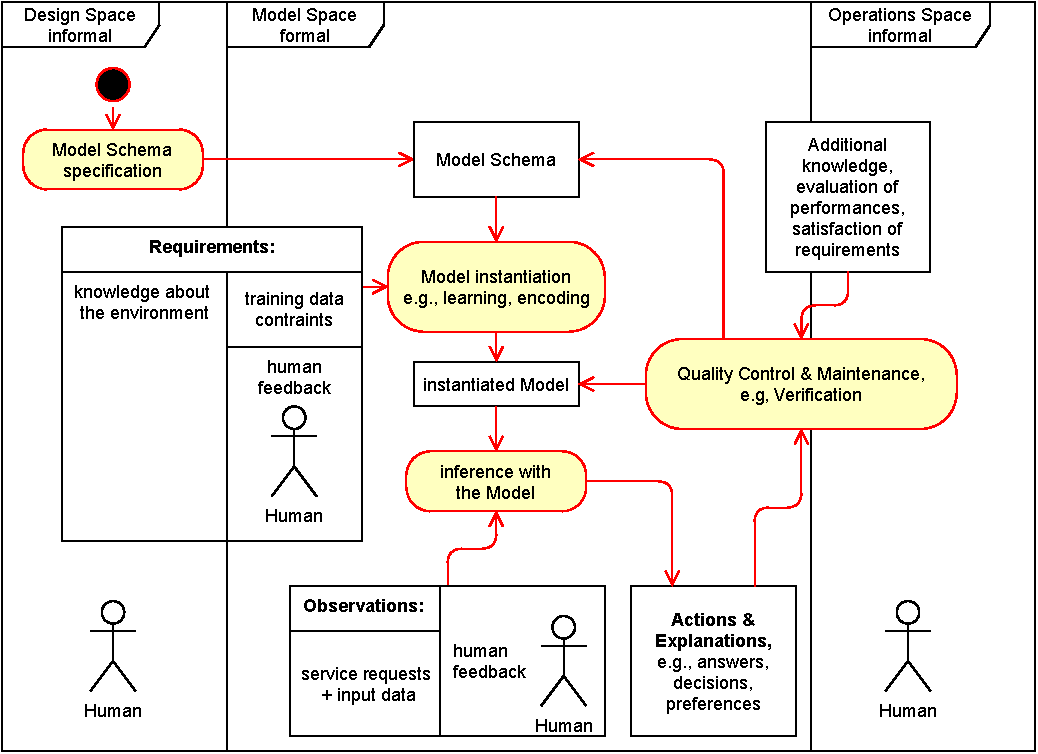
\includegraphics[width=\linewidth]{HCAI-lifecycle-v1}
    \caption{Lifecycle by Peter (v1)}
    \label{fig:peterlifecycle}
\end{figure}
